% Created 2019-05-24 Fri 17:54
% Intended LaTeX compiler: pdflatex
\documentclass[12pt, a4paper]{article}
\usepackage[utf8]{inputenc}
\usepackage[T1]{fontenc}
\usepackage{graphicx}
\usepackage{grffile}
\usepackage{longtable}
\usepackage{wrapfig}
\usepackage{rotating}
\usepackage[normalem]{ulem}
\usepackage{amsmath}
\usepackage{textcomp}
\usepackage{amssymb}
\usepackage{capt-of}
\usepackage{hyperref}
\usepackage[style=authoryear,natbib]{biblatex}
\setlength\bibitemsep{\baselineskip}
\addbibresource{/Users/guilhermesalome/Dropbox/references.bib}
\usepackage[T1]{fontenc}
\usepackage{lmodern}
\usepackage{amsmath}
\usepackage{mathtools}
\usepackage{multirow}
\usepackage{booktabs}
\usepackage{bbm}
\usepackage{dsfont}
\usepackage[]{algorithm2e}
\newcommand\numberthis{\addtocounter{equation}{1}\tag{\theequation}}
\newcommand{\E}[1]{\mathbb{E}{\left[#1\right]}}
\newcommand{\EQ}[1]{\mathbb{E}_t^{\mathbb{Q}}{\left[#1\right]}}
\newcommand{\EP}[1]{\mathbb{E}_t^{\mathbb{P}}{\left[#1\right]}}
\newcommand{\e}[1]{\text{e}^{#1}}
\newcommand{\abs}[1]{\left\vert{#1}\right\vert}
\newcommand{\dis}{\overset{d}{\sim}}
\newcommand{\Var}[1]{\mathrm{Var}\left(#1\right)}
\newcommand{\Corr}[1]{\mathrm{Corr}\left(#1\right)}
\newcommand{\Normal}[1]{\mathcal{N}\left(0, #1\right)}
\newcommand{\Max}[1]{\text{max}\left\{#1\right\}}
\newcommand{\Set}[1]{\left\{#1\right\}}
\renewcommand{\ln}[1]{\text{ln}\left(#1\right)}
\DeclareMathOperator*{\argmin}{\arg\!\min}
\DeclareMathOperator*{\argmax}{\arg\!\max}
\DeclarePairedDelimiter\ceil{\lceil}{\rceil}
\DeclarePairedDelimiter\floor{\lfloor}{\rfloor}
\newcommand{\Poisson}[1]{\text{Poisson}\left(#1\right)}
\newcommand{\Uniform}[1]{\text{Unif}#1}
\newcommand{\Cov}[1]{\mathrm{Cov}\left(#1\right)}
\newtheorem{problem}{Problem}
\usepackage[hang,small,bf]{caption}
\usepackage[margin=1in]{geometry}
\usepackage{mathtools}
\usepackage{xcolor}
\usepackage{resizegather}
\usepackage{multirow}
\definecolor{darkgreen}{rgb}{0.1, 0.6, 0.1}
\usepackage{float}
\usepackage{fancyhdr}
\pagestyle{fancy}
\fancypagestyle{plain}{}
\fancyhf{}
\rfoot{Page \thepage}
\usepackage{ifthen}
\rhead{\ifthenelse{\value{page}=1}{Guilherme Salom\'{e}}{Summer \the\year}}
\lhead{\ifthenelse{\value{page}=1}{Econ890-01 Matlab}{Econ890-01 Matlab}}
\usepackage[numbered,framed]{matlab-prettifier}
\usepackage{listings}
\date{}
\title{Numerical Methods and Symbolic Math}
\hypersetup{
 pdfauthor={Guilherme Salomé},
 pdftitle={Numerical Methods and Symbolic Math},
 pdfkeywords={},
 pdfsubject={},
 pdfcreator={Emacs 26.1 (Org mode 9.2.1)},
 pdflang={English}}
\begin{document}

\maketitle
Consider a simple economic model of consumption, where an agent decides between consumption and investment in capital while maximizing his utility:
\begin{align*}
  \max&\sum_{t=0}^{\infty}\beta^tU(c_t)\\
  \text{subject to }&
                      \begin{cases}
                        c_t = k_t - k_{t+1}, \forall t >= 0\\
                        k_0 > 0
                      \end{cases}
\end{align*}
where \(c_t\) is the time \(t\) consumption, \(k_t\) is the return of the capital invested at \(t-1\) and \(k_{t+1}\) is the investment choice at time \(t\).
In this simple model there is no rate of return in capital, nor depreciation.

We can transform this problem into a recursive problem using Bellman's equation:
\begin{equation*}
\begin{aligned}
V(k) = & \underset{k'}{\text{max}} & & {U(c) + \beta V(k')}\\
& \text{s.t.:} & & c = k - k'
\end{aligned}
\end{equation*}
And we wish to find a solution for the optimal \(c\) and \(k'\) given the previous investment \(k\):
\begin{align*}
c &= g^c(k)\\
k'&= g^k(k)
\end{align*}
We can find the optimal policies \(g^c\) and \(g^k\) by solving the Bellman equation.
Solving the problem requires either approximating the value function or obtaining the Euler equation and then approximating \(c\).
In either case, we need to approximate functions to solve the problem.
We can approximate functions either locally, around a specific point, or globally, over the entire domain of the function.

This lecture discusses methods for approximating functions and how to use them in Matlab.
If we also consider a economic model of consumption where there is uncertainty regarding future states of the economy, then we will notice that to solve the maximization problem we will need to integrate functions.
Therefore, this lecture also discusses methods for integrating functions and the implementations available in Matlab.
We will also discuss the symbolic math capabilities of Matlab, which can help with deriving the equations we need to approximate.
\section{Approximating Functions}
\label{sec:org68f9387}
Given a function \(f\) we want to approximate it by a finite number \(n\) of basis functions \(\Set{p_k}_{k=1}^n\).
We need to choose weights such that:
\begin{align*}
  f(x)&\approx \beta_1 p_1(x) + \beta_2 p_2(x) + \cdots + \beta_n p_n(x)\\
      &=\underbrace{\begin{pmatrix}
        p_1(x) & p_2(x) & \cdots & p_n(x)
      \end{pmatrix}}_{p(x)'}\underbrace{\begin{pmatrix}
        \beta_1\\
        \beta_2\\
        \vdots\\
        \beta_n
      \end{pmatrix}}_{\beta}\\
  &=p(x)'\beta
\end{align*}
If we have a set of points \(\Set{x_i}_{i=1}^d\) where we know the value of \(f\), then we can write:
\begin{align*}
  \underbrace{\begin{pmatrix}
    f(x_1)\\
    f(x_2)\\
    \vdots\\
    f(x_d)
  \end{pmatrix}}_{F}\approx
  \underbrace{\begin{pmatrix}
    p_1(x_1) & p_2(x_1) & \cdots & p_n(x_1)\\
    p_1(x_2) & p_2(x_2) & \cdots & p_n(x_2)\\
    & & \vdots & \\
    p_1(x_d) & p_2(x_d) & \cdots & p_n(x_d)\\
  \end{pmatrix}}_{P}
  \underbrace{\begin{pmatrix}
    \beta_1\\
    \beta_2\\
    \vdots\\
    \beta_d
  \end{pmatrix}}_{\beta}\numberthis{}\label{eq:890_matlab_FPbeta}
\end{align*}
If the number of basis functions and the number of points is the same, that is \(n=d\), then there is an exact solution for \(\beta\) if \(P\) is invertible: \(\beta=P^{-1}F\).

If we have more points than basis functions, then we can compute a least-squares approximation to \(f\):
\begin{align*}
\hat{\beta} \equiv \argmin_{\beta\in\mathbb{R}^n}{\sum_{i=1}^d(f(x_i) - p(x_i)'\beta)^2}\numberthis{}\label{eq:890_matlab_sieves_problem}
\end{align*}
We know that the "OLS" solution is:
\begin{align*}
\hat{\beta}=(P'P)^{-}P'F\numberthis{}\label{eq:890_matlab_ols_solution}
\end{align*}
Notice the use of a \href{https://en.wikipedia.org/wiki/Moore–Penrose\_inverse}{generalized inverse} in \((P'P)^{-}\).
This is necessary because depending on choice of the basis function, we might have a column of zeros in \(P\) (this happens with splines when there are more knots relative to points).
Now, the function that approximates \(f\) is:
\begin{align*}
\hat{f}(x) \equiv p(x)'\hat{\beta}\numberthis{}\label{eq:890_matlab_fhat}
\end{align*}
This approximating function can be computed given a choice of basis functions \(\Set{p_k}_{k=1}^n\) and a collection of data points \(\Set{x_i}_{i=1}^d\).

As an aside, consider the case where the original function we wanted to estimate was a conditional mean, \(f(x)=\E{Y\vert X=x}\).
If we have i.i.d. observations of \(f\) and \(x\), then the \(\hat{f}\) above is exactly the non-parametric Sieves estimator for the conditional mean.
In this case, there is theory justifying the consistency and asymptotic normality of \(\hat{f}\).

Next, we discuss the possible choices for basis functions.
\subsection{Jacobi Polynomials}
\label{sec:orge3f4007}
The \href{https://en.wikipedia.org/wiki/Jacobi\_polynomials\#Orthogonality}{Jacobi polynomials} are a family of orthogonal polynomials defined over the interval \([-1, 1]\).
Let's denote the family of Jacobi polynomials by \(\mathcal{P}\), and the members of this family by \(P_n^{(\alpha,\beta)}\) (to be defined later), where \(n\) denotes the highest degree of the polynomial.
The Jacobi polynomials are parameterized by \(\alpha\) and \(\beta\), which satisfy \(\alpha>-1\) and \(\beta>-1\).

We say that a family of polynomials is orthogonal if any two of its members are orthogonal to each other under some inner product.
In the case of Jacobi polynomials, there is a weight function \(w\) such that \(\forall P_n^{(\alpha, \beta)}, P_m^{(\alpha, \beta)} \in\mathcal{P}\):
\begin{align*}
\int w(x)P_n^{(\alpha, \beta)}(x) P_m^{(\alpha, \beta)}(x)dx = 0 \text{ if } n\neq m
\end{align*}

The Jacobi polynomials are defined as (see Equation 22.3.1 in \citet{AS1964}):
\begin{align*}
P_n^{(\alpha, \beta)}=\frac{1}{2^n}\sum_{m=0}^n\binom{n+\alpha}{m}\binom{n+\beta}{n-m}(x-1)^{n-m}(x+1)^m
\end{align*}
These polynomials are orthogonal with respect to the weight function:
\begin{align*}
w^{(\alpha, \beta)}\equiv (1-x)^{\alpha}(1+x)^{\beta}
\end{align*}

The Jacobi polynomials are available in Matlab's \href{https://www.mathworks.com/help/symbolic/index.html?s\_tid=CRUX\_lftnav}{Symbolic Math Toolbox} via the function \href{https://www.mathworks.com/help/symbolic/jacobip.html}{\texttt{jacobiP}}.
This function evaluates the Jacobi polynomial of degree \(n\) and parameters \((\alpha, \beta)\) at a point \(x\).
We can plot the functions to get a sense of their shape and of the influence of the parameters \(\alpha\) and \(\beta\):
\lstset{language=matlab,label= ,caption= ,captionpos=b,firstnumber=1,numbers=left,style=Matlab-editor}
\begin{lstlisting}
% read documentation
help jacobiP
% create a jacobi polynomial for different degrees
alpha = 1;
beta = 1;
jacobi = @(k, x) jacobiP(k, alpha, beta, x);
% graph a few of the polynomials
fig = figure;
hold on;
for k = 1:5
    fplot(@(x) jacobi(k, x), [-1, 1]);
end
% compare changes in alpha
figure;
hold on;
for alpha = [-0.5, 0, 0.5, 1, 2]
    jp = @(x) jacobiP(3, alpha, 1, x);
    fplot(jp, [-1, 1]);
end
legend(["$\alpha=-0.5$", "$\alpha=0$", "$\alpha=0.5$", "$\alpha=1$", ...
        "$\alpha=2$"], 'Interpreter', 'latex', ...
       'location', 'southeastoutside');
% compare changes in beta
figure;
hold on;
for beta = [-0.5, 0, 0.5, 1, 2]
    jp = @(x) jacobiP(3, 1, beta, x);
    fplot(jp, [-1, 1]);
end
legend(["$\beta=-0.5$", "$\beta=0$", "$\beta=0.5$", "$\beta=1$", ...
        "$\beta=2$"], 'Interpreter', 'latex', ...
       'location', 'southeastoutside');
\end{lstlisting}
We can verify that the Jacobi polynomials are indeed orthogonal:
\lstset{language=matlab,label= ,caption= ,captionpos=b,firstnumber=1,numbers=left,style=Matlab-editor}
\begin{lstlisting}
alpha = 1;
beta = 1;
jacobi = @(k, x) jacobiP(k, alpha, beta, x);
% verify orthogonality
w = @(x) (1-x).^alpha.*(1+x).^beta;
integral(@(x) (w(x).*jacobi(2, x).*jacobi(4, x)), -1, 1)
% what about orthonormality?
integral(@(x) (w(x).*jacobi(2, x).*jacobi(2, x)), -1, 1)
\end{lstlisting}
\subsubsection{Expanding the Domain}
\label{sec:orgfe2f8f7}
The Jacobi polynomials are initially defined over \([-1, 1]\), but we can extend the domain to some compact interval \([a, b]\) via a linear change of variables:
\begin{align*}
y = -1 + 2\frac{x-a}{b-a}
\end{align*}
In this case, we can write the polynomials as:
\begin{align*}
\tilde{P}_k^{(\alpha, \beta)}(x) = P_k^{(\alpha, \beta)}\left(-1 + 2\frac{x-a}{b-a}\right)
\end{align*}
These polynomials are now orthogonal with respect to a different weight function:
\begin{align*}
\tilde{w}^{(\alpha, \beta)} = (b-x)^{\alpha}(x-a)^{\beta}
\end{align*}
Indeed:
\lstset{language=matlab,label= ,caption= ,captionpos=b,firstnumber=1,numbers=left,style=Matlab-editor}
\begin{lstlisting}
% extend jacobi polynomial to [a, b]
alpha = 1;
beta = 1;
a = 0;
b = 100;
jacobi = @(k, x) jacobiP(k, alpha, beta, -1+2.*(x-a)./(b-a));
% modified weight function
w = @(x) (b-x).^alpha.*(x-a).^beta;
% orthogonality
integral(@(x) (w(x).*jacobi(2, x).*jacobi(3, x)), -1, 1) % wrong domain
integral(@(x) (w(x).*jacobi(2, x).*jacobi(3, x)), a, b)
\end{lstlisting}
\subsubsection{Orthonormal Jacobi Polynomials}
\label{sec:org3f85b13}
It is also possible to make the Jacobi polynomials orthonormal, instead of just orthogonal.
We just need to scale the polynomials by a constant that depends on the degree of the polynomial, on the parameters \(\alpha\) and \(\beta\), and on the length of the domain.

We can define the orthonormal Jacobi polynomials as:
\begin{align*}
\tilde{P}_k^{(\alpha, \beta)}(x) &\equiv c^{(\alpha, \beta)}(k)P_k^{(\alpha, \beta)}\left(-1+2\frac{x-a}{b-a}\right)\\
c^{(\alpha, \beta)}(k)&\equiv \left(\frac{1}{b-a}\right)^{\frac{\alpha+\beta+1}{2}}\sqrt{\frac{(2k+\alpha+\beta+1)\Gamma(k+1)\Gamma(k+\alpha+\beta+1)}{\Gamma{(k+\alpha+1)}\Gamma{(k+\beta+1)}}}
\end{align*}
Where \(\Gamma\) is the \href{https://en.wikipedia.org/wiki/Gamma\_function}{Gamma function}, which is available in Matlab via the function \href{https://www.mathworks.com/help/symbolic/gamma.html?.mathworks.com}{\texttt{gamma}}.
These polynomials are orthonormal with respect to the weight function:
\begin{align*}
\tilde{w}^{(\alpha, \beta)} = (b-x)^{\alpha}(x-a)^{\beta}
\end{align*}
We can verify the orthonormality of the Jacobi polynomials defined by \(\tilde{P}_k^{(\alpha, \beta)}(x)\):
\lstset{language=matlab,label= ,caption= ,captionpos=b,firstnumber=1,numbers=left,style=Matlab-editor}
\begin{lstlisting}
a = 0;
b = 10;
alpha = 1;
beta = 1;
% define weight function
w = @(x) ((b-x).^alpha).*((x-a).^beta);
% define scaling constant
c = @(k) ((1/(b-a))^((alpha+beta+1)/2)).*((((2.*k+alpha+beta+1).*gamma(k+1).*gamma(k+alpha+beta+1))./(gamma(k+alpha+1).*gamma(k+beta+1))).^0.5);
% define orthonormal jacobi function
jacobi = @(k, x) (c(k).*jacobiP(k, alpha, beta, -1 + 2.*(x-a)./(b-a)));
% visualize
fig = figure;
hold on;
for k = 1:5
    fplot(@(x) jacobi(k, x), [a, b]);
end
% check orthonormality
integral(@(x) (w(x).*jacobi(2, x).*jacobi(3, x)), a, b) % 0
integral(@(x) (w(x).*jacobi(2, x).*jacobi(2, x)), a, b) % 1
\end{lstlisting}
\subsubsection{Special Case: Legendre Polynomials}
\label{sec:org43326d9}
The \href{https://en.wikipedia.org/wiki/Legendre\_polynomials}{Legendre} polynomials are special cases of Jacobi polynomials.
We can obtain Legendre polynomials by setting \(\alpha=\beta=0\).
In this case we have:
\begin{align*}
P_k^{(0, 0)}(x) &= \frac{1}{2^k}\sum_{m=0}^k{\binom{k}{m}}^2(x-1)^{k-m}(x+1)^m\\
c^{(0, 0)}&=\sqrt{\frac{2k+1}{b-a}}\\
L_k(x)&\equiv \tilde{P}_k^{(0, 0)}(x)=c^{(0, 0)}(k)P_k^{(0, 0)}\left(-1+2\frac{x-a}{b-a}\right)
\end{align*}
Notice that the weight function for the Legendre polynomials is simply 1.

The Legendre polynomials can also be computed recursively:
\begin{align*}
{P}_0^{(0, 0)}(x) &= 1\\
{P}_1^{(0, 0)}(x) &= x\\
{P}_k^{(0, 0)}(x) &= \left(x\cdot\frac{2k-1}{k}\right){P}_{k-1}^{(0, 0)}(x) + \left(\frac{k-1}{k}\right){P}_{k-2}^{(0, 0)}(x)
\end{align*}
Notice that the recursion is for the orthogonal Legendre polynomials defined over \([-1, 1]\).
We can extend the recursion to the orthonormal Legendre polynomials by simply multiplying the \(P_k^{(0, 0)}\) above by the scaling constant \(c^{(0, 0)}(k)\).

We can obtain the Legendre polynomials in Matlab via the function \href{https://www.mathworks.com/help/symbolic/legendrep.html?s\_tid=doc\_ta\#buei9e5-6}{\texttt{legendreP}}.
This function is similar to \texttt{jacobiP} and evaluates the Legendre polynomial of degree \(n\) at the point \(x\).
\lstset{language=matlab,label= ,caption= ,captionpos=b,firstnumber=1,numbers=left,style=Matlab-editor}
\begin{lstlisting}
% define interval [a, b]
a = 0;
b = 10;
% define scaling constant
c = @(k) ((2.*k+1)./(b-a)).^0.5;
% define orthonormal legendre polynomials
lp = @(k, x) c(k).*legendreP(k, -1 + 2.*(x-a)./(b-a));
% check orthonormality (good for catching bugs)
l1 = @(x) lp(1, x);
l2 = @(x) lp(2, x);
integral(@(x) l1(x).*l2(x), a, b)       % 0
integral(@(x) l2(x).*l2(x), a, b)       % 1
\end{lstlisting}
Let's visualize the first few Legendre polynomials:
\lstset{language=matlab,label= ,caption= ,captionpos=b,firstnumber=1,numbers=left,style=Matlab-editor}
\begin{lstlisting}
a = -1;
b = 1;
% define scaling constant
c = @(k) ((2.*k+1)./(b-a)).^0.5;
% define orthonormal legendre polynomials
lp = @(k, x) c(k).*legendreP(k, -1 + 2.*(x-a)./(b-a));
% visualize the basis
f = figure;
for k = 1:6
    subplot(2, 3, k)
    fplot(@(x) lp(k, x), [a b]);
    grid on;
    legend(strcat("$L_", string(k), "(x)$"), 'Interpreter', 'latex');
end
\end{lstlisting}
Figure \ref{fig:orgd8f8da3} displays the orthonormal Legendre polynomials.
\begin{figure}[H]
\centering
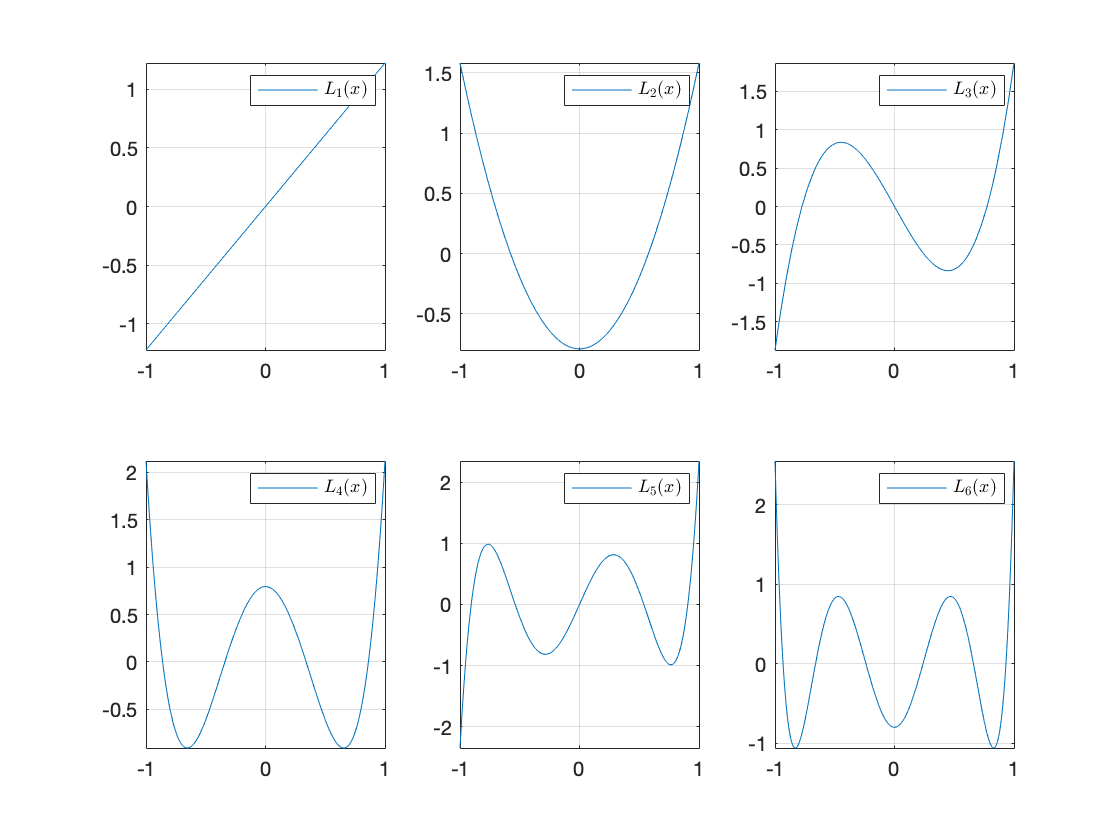
\includegraphics[width=8cm]{/Users/guilhermesalome/Teaching/Duke/Econ890 Matlab - 2019/supporting/matlab_legendre_basis.png}
\caption{\label{fig:orgd8f8da3}
Orthonomal Legendre Polynomials.}
\end{figure}
\subsubsection{Special Case: Chebyshev Polynomials}
\label{sec:org5be0814}
The \href{https://en.wikipedia.org/wiki/Chebyshev\_polynomials}{Chebyshev} polynomials are also a special case of the Jacobi polynomials.
There are two families of Chebyshev polynomials depending on the values of \(\alpha\) and \(\beta\).
If we set \(\alpha=\beta=-\frac{1}{2}\), then we get the Chebyshev polynomials of the first kind, denoted by \(T_k(x)\).
If we set \(\alpha=\beta=\frac{1}{2}\), then we get the Chebyshev polynomials of the second kind, denoted by \(U_k(x)\).

These polynomials can be computed recursively.
For the first kind, we have:
\begin{align*}
T_0(x)&\equiv P_0^{(-0.5, -0.5)}=1\\
T_1(x)&\equiv P_1^{(-0.5, -0.5)}=x\\
T_k(x)&\equiv 2xT_{k-1}(x)-T_{k-2}(x)
\end{align*}

For the second kind, we have:
\begin{align*}
U_0(x)&\equiv P_0^{(0.5, 0.5)}=1\\
U_1(x)&\equiv P_1^{(0.5, 0.5)}=2x\\
U_k(x)&\equiv 2xU_{k-1}(x)-U_{k-2}(x)
\end{align*}

The Chebyshev polynomials are available in the functions \href{https://www.mathworks.com/help/symbolic/chebyshevt.html}{\texttt{chebyshevT}} (first kind) and \href{https://www.mathworks.com/help/symbolic/chebyshevu.html?s\_tid=doc\_ta}{\texttt{chebyshevU}} (second kind).
\lstset{language=matlab,label= ,caption= ,captionpos=b,firstnumber=1,numbers=left,style=Matlab-editor}
\begin{lstlisting}
a = -1;
b = 1;
% define weight function
wT = @(x) ((b-x).*(x-a)).^(-0.5);
% orthogonality of chebyshev polynomials
integral(@(x) wT(x).*chebyshevT(2, x).*chebyshevT(3, x), a, b)
integral(@(x) wT(x).*chebyshevT(3, x).*chebyshevT(3, x), a, b)

% define constant for orthonormality
cT = @(k) (2.*k.*gamma(k+1).*gamma(k)./(gamma(k+0.5).*gamma(k+0.5))).^(0.5);
% define orthonormal chebyshev polynomials
orthoC = @(k, x) cT(k).*jacobiP(k, -0.5, -0.5, -1 + 2.*(x-a)./(b-a));
% orthonormality
integral(@(x) wT(x).*orthoC(2, x).*orthoC(3, x), a, b)
integral(@(x) wT(x).*orthoC(2, x).*orthoC(2, x), a, b)
\end{lstlisting}

Let's visualize the first few orthonormal Chebyshev (first kind) polynomials:
\lstset{language=matlab,label= ,caption= ,captionpos=b,firstnumber=1,numbers=left,style=Matlab-editor}
\begin{lstlisting}
f = figure;
for k = 1:6
    subplot(2, 3, k)
    fplot(@(x) orthoC(k, x), [a b]);
    grid on;
    legend(strcat("$T_", string(k), "(x)$"), 'Interpreter', 'latex');
end
\end{lstlisting}
Figure \ref{fig:orgb14ac18} displays the orthonormal Legendre polynomials.
\begin{figure}[H]
\centering
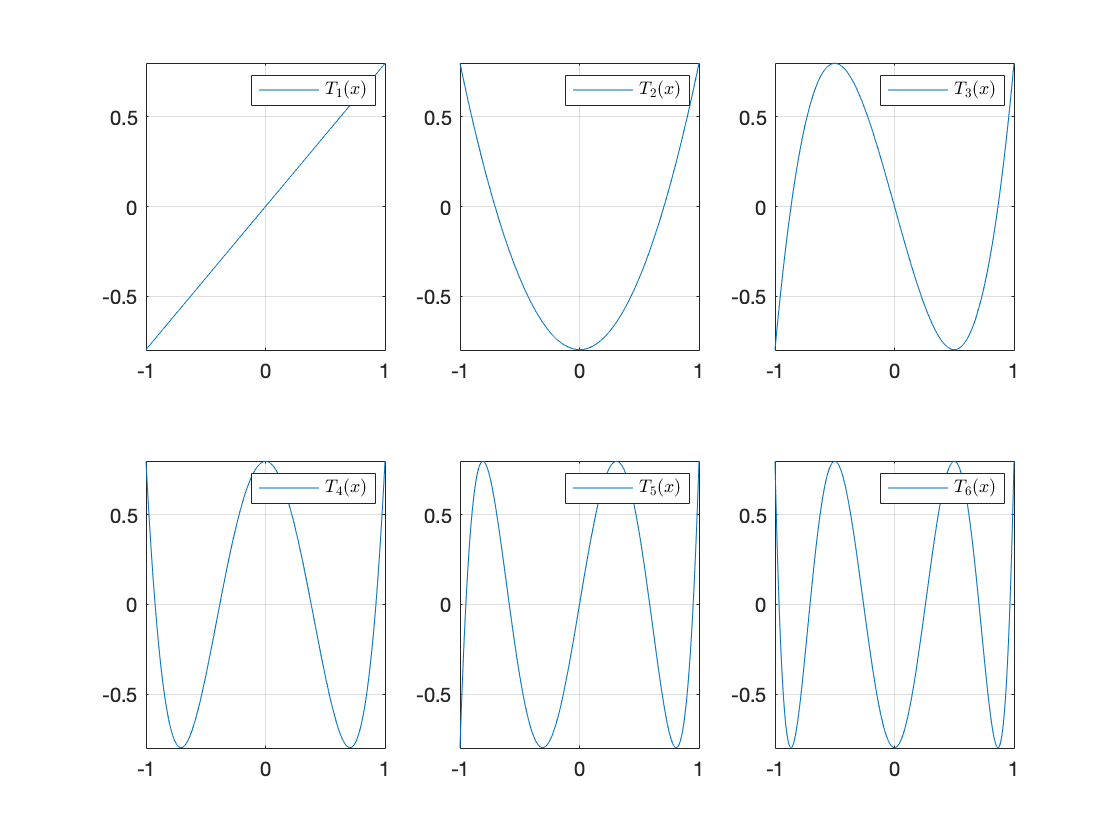
\includegraphics[width=8cm]{/Users/guilhermesalome/Teaching/Duke/Econ890 Matlab - 2019/supporting/matlab_chebyshev_first_kind_basis.png}
\caption{\label{fig:orgb14ac18}
Orthonomal Chebyshev Polynomials (first kind).}
\end{figure}
\subsubsection{Example}
\label{sec:org1064d54}
Let's approximate the logistic function:
\begin{align*}
f(x)=\frac{1}{1+\e{-x}}
\end{align*}
To approximate \(f\), we need to choose a basis of polynomials.
In this example, we will use the orthonormal Legendre polynomials.
We also need to compute the generalized inverse of the matrix \(P'P\).
In Matlab, the generalized inverse (Moore-Penrose) of a matrix can be computed with the function \href{https://www.mathworks.com/help/matlab/ref/pinv.html?s\_tid=doc\_ta}{\texttt{pinv}}.
\lstset{language=matlab,label= ,caption= ,captionpos=b,firstnumber=1,numbers=left,style=Matlab-editor}
\begin{lstlisting}
% consider the logistic function
f = @(x) 1./(1+exp(-x));
% consider 5 points
x = linspace(-5, 5, 5)';
% select a basis of polynomials: orthonormal Legendre polynomials
% use 2 polynomials
c = @(k) ((2.*k+1)./(b-a)).^0.5;
p = @(x) [c(0).*legendreP(0, x) c(1).*legendreP(1, x)];
% visualize basis
fplot(p, [-5 5]);
% compute the matrices F, P and the generalized inverse of P'P
F = f(x);
P = p(x);
beta = pinv(P'*P)*P'*F;
% approximation for the function f
fhat = @(x) p(x)*beta;
% compare original to approximation
fplot(f);
hold on;
fplot(fhat);
\end{lstlisting}

We can make the approximation more precise by increasing the number of polynomials.
\lstset{language=matlab,label= ,caption= ,captionpos=b,firstnumber=1,numbers=left,style=Matlab-editor}
\begin{lstlisting}
% use 4 polynomials
p = @(x) [c(0).*legendreP(0, x) c(1).*legendreP(1, x) ...
          c(2).*legendreP(2, x) c(3).*legendreP(3, x)];
F = f(x);
P = p(x);
beta = pinv(P'*P)*P'*F;
% approximation for the function f
fhat = @(x) p(x)*beta;
% compare original to approximation
fplot(f);
hold on;
fplot(fhat);
\end{lstlisting}

At this point there are a few observations to be made.
First, coding the polynomials by hand is surprisingly hard, since it is quite easy to make mistakes but hard to debug.
If you ever need to do so, the orthogonality and orthonomality conditions are useful to check if everything is correct.
Second, the approximation of continuous functions over compacts is justified by \href{https://en.wikipedia.org/wiki/Jackson\%27s\_inequality}{Jackson's theorems}.
Third, better approximations require a higher number of basis functions.
Fourth, to approximate more complex functions you need a higher number of \((x, f(x))\) observations.
\subsection{Hermite Polynomials}
\label{sec:org086448e}
The Jacobi polynomials are defined to be orthogonal on a compact interval.
The motivation for Hermite polynomials is to find a family of polynomials that is orthogonal on the real line.
We can define \href{https://en.wikipedia.org/wiki/Hermite\_polynomials}{Hermite polynomials} recursively.
Let \(H_k\) denote the Hermite polynomial of order \(k\), then:
\begin{align*}
H_0(x)&\equiv 1\\
H_1(x)&\equiv 2x\\
H_k(x)&\equiv 2xH_{k-1}(x)-2(k-1)H_{k-2}(x)
\end{align*}

The Hermite polynomials are orthogonal on the real line with respect to the weight function:
\begin{align*}
w(x) = \e{-x^2}
\end{align*}
In Matlab, Hermite polynomials can be computed with the function \href{https://www.mathworks.com/help/symbolic/hermiteh.html}{\texttt{hemiteH}}:
\lstset{language=matlab,label= ,caption= ,captionpos=b,firstnumber=1,numbers=left,style=Matlab-editor}
\begin{lstlisting}
% visualize
figure;
hold on;
for k = 3:5
    fplot(@(x) hermiteH(k, x));
end
% weight function
w = @(x) exp(-x.^2);
% verify orthogonality
integral(@(x) w(x).*hermiteH(2, x).*hermiteH(1, x), -Inf, Inf)
integral(@(x) w(x).*hermiteH(2, x).*hermiteH(2, x), -Inf, Inf)
\end{lstlisting}
It is possible to show that:
\begin{align*}
\int_{-\infty}^{\infty}w(x)H_k(x)H_k(x)dx=2^kk!\sqrt{\pi}
\end{align*}
Thus, we can define Hermite polynomials that are orthonormal and with weight function \(w(x)=1\), by defining:
\begin{align*}
\tilde{H}_k(x)&=\sqrt{\frac{w(x)}{2^kk!\sqrt{\pi}}}H_k(x)\\
&=(2^kk!\sqrt{\pi})^{-\frac{1}{2}}\e{-\frac{x^2}{2}}H_k(x)
\end{align*}
The family of polynomials \(\Set{\tilde{H}_k:k\in\mathbb{N}\cup\Set{0}}\) is orthonormal.
\lstset{language=matlab,label= ,caption= ,captionpos=b,firstnumber=1,numbers=left,style=Matlab-editor}
\begin{lstlisting}
% build the orthonormal hermite polynomials
orthoH = @(k, x) hermiteH(k, x)./((2^k*factorial(k)*sqrt(pi).*exp(x.^2)).^(0.5));
% verify orthonormality (good way to debug)
integral(@(x) orthoH(2, x).*orthoH(3, x), -Inf, Inf)
integral(@(x) orthoH(3, x).*orthoH(3, x), -Inf, Inf)
\end{lstlisting}

Let's visualize the first few orthonormal Hermite polynomials:
\lstset{language=matlab,label= ,caption= ,captionpos=b,firstnumber=1,numbers=left,style=Matlab-editor}
\begin{lstlisting}
f = figure;
for k = 1:6
    subplot(2, 3, k)
    fplot(@(x) orthoH(k, x), [-5 5]);
    grid on;
    legend(strcat("$H_", string(k), "(x)$"), 'Interpreter', 'latex');
end
\end{lstlisting}
Figure \ref{fig:org3726ce7} displays the first few orthonormal Hermite polynomials.
\begin{figure}[H]
\centering
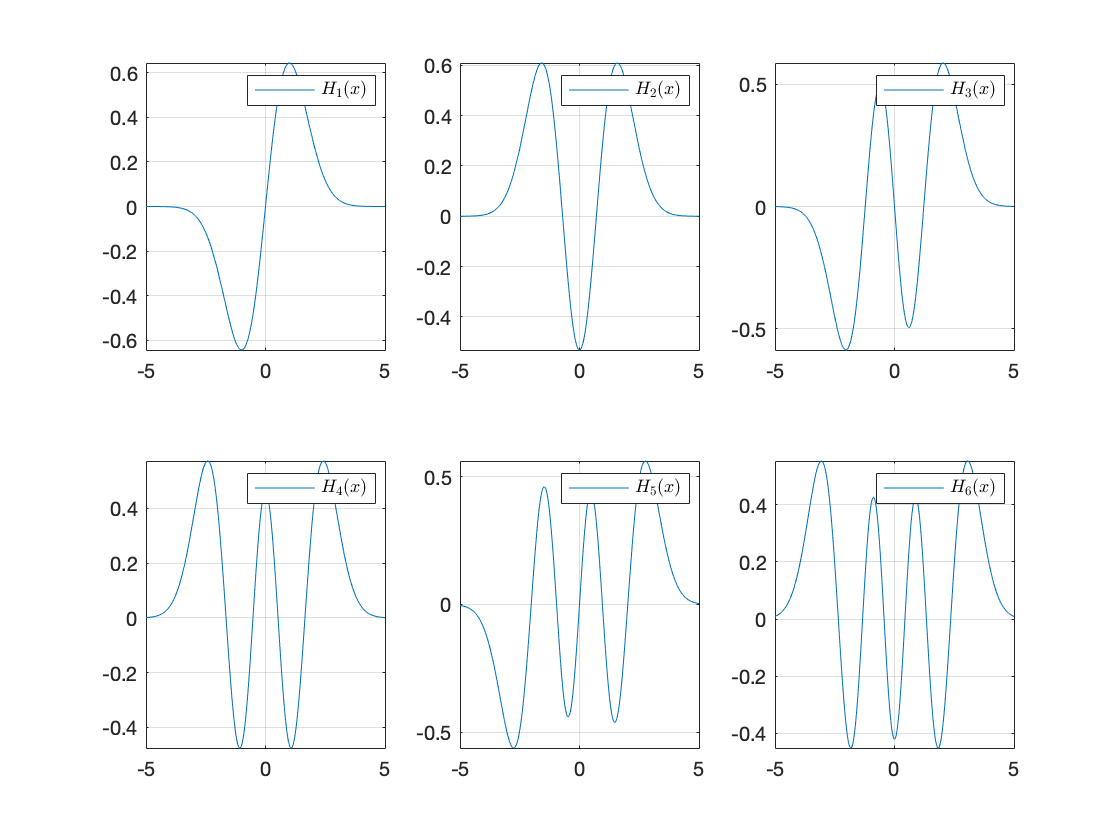
\includegraphics[width=8cm]{/Users/guilhermesalome/Teaching/Duke/Econ890 Matlab - 2019/supporting/matlab_hermite_basis.png}
\caption{\label{fig:org3726ce7}
Orthonomal Hermite Polynomials.}
\end{figure}
\subsubsection{Example}
\label{sec:org4110795}
Let's approximate the density of the Cauchy distribution:
\begin{align*}
f(x; x_0, \gamma)&=\frac{1}{\pi\gamma\left[1+\left(\frac{x-x_0}{\gamma}\right)^2\right]}
\end{align*}
To approximate \(f\), we need to choose a basis of polynomials.
In this example, we will use the orthonormal Hermite polynomials.
\lstset{language=matlab,label= ,caption= ,captionpos=b,firstnumber=1,numbers=left,style=Matlab-editor}
\begin{lstlisting}
% consider the cauchy density
x0 = -2;
gamma = 1;
f = @(x) 1./((pi*gamma)*[1+((x-x0)/gamma).^2]);
% consider 5 points
x = linspace(-5, 5, 5)';
% select a basis of polynomials: orthonormal Hermite polynomials
% use 2 polynomials
p = @(x) [orthoH(0, x) orthoH(1, x)];
% visualize basis
fplot(p, [-5 5]);
% compute the matrices F, P and the generalized inverse of P'P
F = f(x);
P = p(x);
beta = pinv(P'*P)*P'*F;
% approximation for the function f
fhat = @(x) p(x)*beta;
% compare original to approximation
fplot(f);
hold on;
fplot(fhat);
grid on;
legend(["f", "$\hat{f}$"], 'interpreter', 'latex');
\end{lstlisting}

To improve the approximation, we need more observations of the function we want to approximate and to increase the number of basis polynomials.
\lstset{language=matlab,label= ,caption= ,captionpos=b,firstnumber=1,numbers=left,style=Matlab-editor}
\begin{lstlisting}
x = linspace(-5, 5, 1000)';
% use 4 polynomials
p = @(x) [orthoH(0, x) orthoH(1, x) orthoH(2, x) ...
          orthoH(3, x) orthoH(4, x) orthoH(5, x) ...
          orthoH(6, x) orthoH(7, x) orthoH(8, x)];
F = f(x);
P = p(x);
beta = pinv(P'*P)*P'*F;
% approximation for the function f
fhat = @(x) p(x)*beta;
% compare original to approximation
fplot(f, [-5 5]);
hold on;
plot(x, fhat(x));
grid on;
legend(["$f$", "$\hat{f}$"], 'interpreter', 'latex');
\end{lstlisting}
\subsection{Laguerre Polynomials}
\label{sec:org4a37d52}
The \href{https://en.wikipedia.org/wiki/Laguerre\_polynomials}{Laguerre polynomials} form a class of orthonormal polynomials on the non-negative real numbers, with the weight function \(w(x)=\e{-x}\).
These polynomials can be defined recursively:
\begin{align*}
L_0(x) &\equiv 1\\
L_1(x) &\equiv 1-x\\
L_k(x) &\equiv \frac{(2k-1-x)L_{k-1}(x)-(k-1)L_{k-2}(x)}{k}
\end{align*}

The function \href{https://www.mathworks.com/help/symbolic/laguerrel.html}{\texttt{laguerreL}} computes the Laguerre polynomial of order \(k\) at a point \(x\):
\lstset{language=matlab,label= ,caption= ,captionpos=b,firstnumber=1,numbers=left,style=Matlab-editor}
\begin{lstlisting}
% weight function
w = @(x) exp(-x);
% orthonormality
integral(@(x) w(x).*laguerreL(3, x).*laguerreL(2, x), 0, Inf)
integral(@(x) w(x).*laguerreL(3, x).*laguerreL(3, x), 0, Inf)
% orthonormal on the non-negative numbers with w(x) = 1
orthoL = @(k, x) laguerreL(k, x).*w(x).^0.5;
integral(@(x) orthoL(3, x).*orthoL(2, x), 0, Inf)
integral(@(x) orthoL(3, x).*orthoL(3, x), 0, Inf)
\end{lstlisting}

Let's visualize the first few orthonormal Laguerre polynomials:
\lstset{language=matlab,label= ,caption= ,captionpos=b,firstnumber=1,numbers=left,style=Matlab-editor}
\begin{lstlisting}
% visualize
figure;
for k = 1:6
    subplot(2, 3, k);
    fplot(@(x) orthoL(k, x), [0 10]);
    grid on;
    legend(strcat("$L_", string(k), "(x)$"), 'Interpreter', 'latex');
end
\end{lstlisting}
Figure \ref{fig:orgb8c55ad} displays the first few orthonormal Laguerre polynomials.
\begin{figure}[H]
\centering
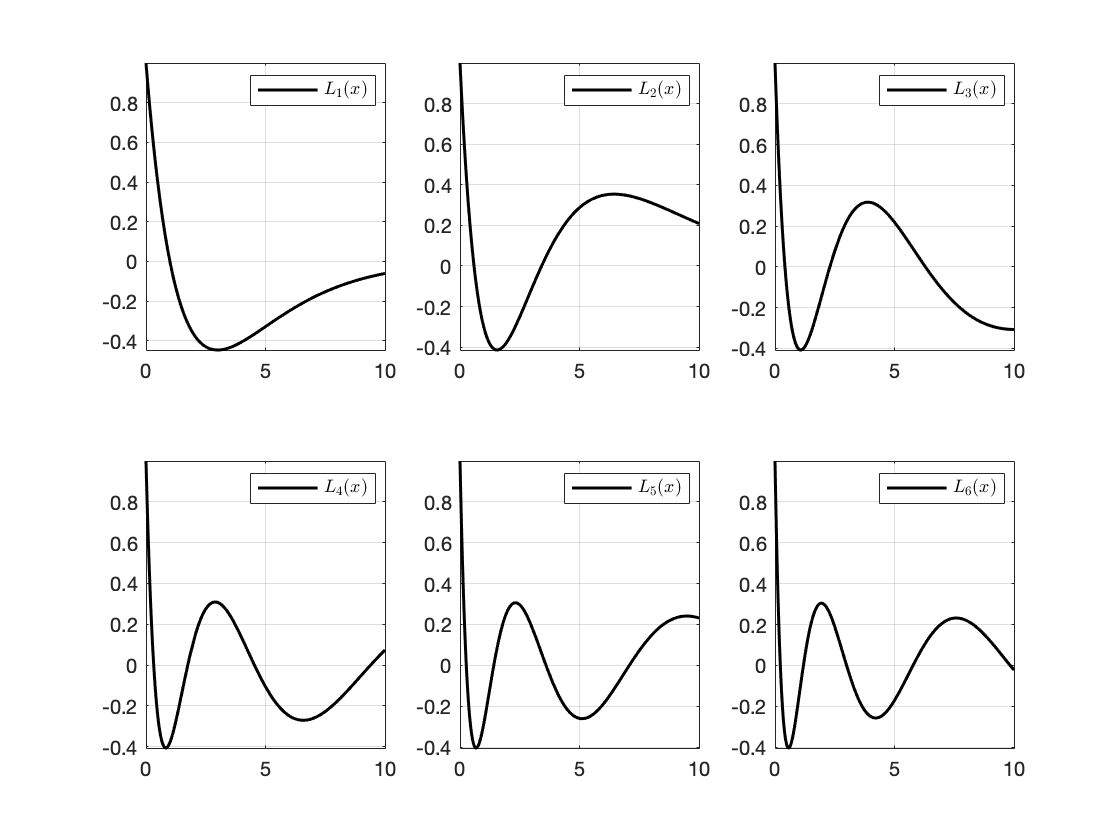
\includegraphics[width=8cm]{/Users/guilhermesalome/Teaching/Duke/Econ890 Matlab - 2019/supporting/matlab_laguerre_basis.png}
\caption{\label{fig:orgb8c55ad}
Orthonomal Laguerre Polynomials.}
\end{figure}
\subsubsection{Example}
\label{sec:org0547eb8}
Let's approximate the density of a Chi-squared distribution:
\begin{align*}
  f(x, v) &\equiv \begin{cases}
    \frac{x^{\frac{k}{2}-1}\e{-\frac{x}{2}}}{2^{\frac{k}{2}}\Gamma\left(\frac{k}{2}\right)},\text{
      if } x > 0\\
    0,\text{ otherwise}
  \end{cases}
\end{align*}
where \(v\) denotes the degrees of freedom of the distribution (also its mean in this case).
We can use the Matlab function \href{https://www.mathworks.com/help/stats/chi2pdf.html?s\_tid=doc\_ta}{\texttt{chi2pdf}} to evaluate the density.
We will use the Laguerre polynomials to approximate the density, since the density of a Chi-squared is defined for non-negative numbers.
\lstset{language=matlab,label= ,caption= ,captionpos=b,firstnumber=1,numbers=left,style=Matlab-editor}
\begin{lstlisting}
% Chi-squared density with 3 degrees of freedom
f = @(x) chi2pdf(x, 3);
% Create orthonormal Laguerre polynomials
w = @(x) exp(-x);
orthoL = @(k, x) laguerreL(k, x).*w(x).^0.5;
p = @(x) [orthoL(0, x) orthoL(1, x) orthoL(2, x)];
% Approximate function
x = [0:5]';
beta = pinv(p(x)'*p(x))*p(x)'*f(x);
fhat = @(x) p(x)*beta;
% Visualize
fplot(f, [0 10]);
hold on;
fplot(fhat, [0 10]);
grid on;
legend(["Chi-squared", "Approximation"]);
\end{lstlisting}
\subsection{Piecewise Polynomials (Splines)}
\label{sec:org1d53b1f}
Polynomials are useful to approximate continuous functions, however the approximations often oscillate wildly.
These oscillations are more apparent at the tails of the function we are approximating.

Consider the approximation of a simple function \(f(x)=\frac{1}{1+x^2}\) over the interval \([-5, 5]\) using polynomials.
The function we want to approximate is infinitely differentiable, but the approximation by polynomials will incur in a wild oscillation near the tails of the function.
This example is known as \href{https://en.wikipedia.org/wiki/Runge\%27s\_phenomenon}{Runge's example}.
\lstset{language=matlab,label= ,caption= ,captionpos=b,firstnumber=1,numbers=left,style=Matlab-editor}
\begin{lstlisting}
% Runge's example: continuous function on interval [-5, 5]
f = @(x) 1./(1+x.^2);
fplot(f, [-5  5]);
% Legrende polynomials
a = -5;
b = 5;
c = @(k) ((2.*k+1)./(b-a)).^0.5;
lp = @(k, x) c(k).*legendreP(k, -1 + 2.*(x-a)./(b-a));
% Approximation using 11 points
x = [-5:5]';
p = @(x) [lp(0, x) lp(1, x) lp(2, x) lp(3, x) lp(4, x) lp(5, x) ...
          lp(6, x) lp(7, x) lp(8, x) lp(9, x) lp(10, x)];
beta = pinv(p(x)'*p(x))*p(x)'*f(x);
fhat = @(x) p(x)*beta;
% Visualize
hold on;
plot(linspace(-5, 5)', fhat(linspace(-5, 5)'));
legend(["Original Function", "Approximation"]);
\end{lstlisting}

Figure \ref{fig:orge3072c0} displays Runge's example.
Notice that the approximation works well around zero, but gets increasingly worse as we move towards the ends of the intervals.
\begin{figure}[H]
\centering
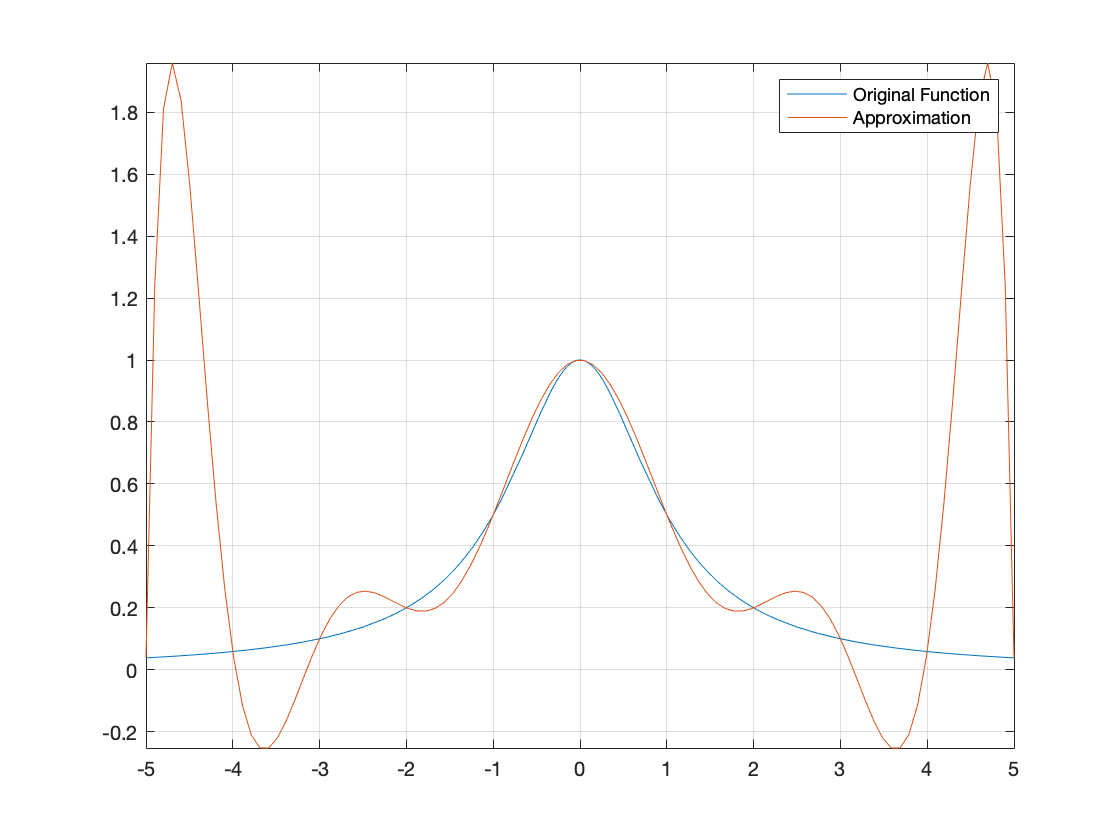
\includegraphics[width=8cm]{/Users/guilhermesalome/Teaching/Duke/Econ890 Matlab - 2019/supporting/matlab_runge_example.png}
\caption{\label{fig:orge3072c0}
Runge's Example.}
\end{figure}

The idea of piecewise polynomials is that instead of using a single polynomial to approximate a function, we could use various different polynomials to approximate different parts of the function.
We say that a function \(s:[a,b]\mapsto\mathbb{R}\) is a \textbf{piecewise polynomial of degree k} if:
\begin{itemize}
\item The function \(s\) is continuous over \([a,b]\);
\item There exists a finite number \(n+1\) of points \(\Set{\xi_i}_{i=1}^{n+1}\), with \(a=\xi_0<\xi_1<\cdots<\xi_n=b\), where \(s\) is a polynomial of degree at most \(k\) on each of the intervals \([\xi_{i-1}, \xi_i], i=1,2,\ldots,n\).
\end{itemize}
That is, \(s\) is a continuous function, but restricted to each interval it is also a polynomial of degree at most \(k\).
The points \(\xi_i\) are called \textbf{knots}.
If the function \(s\) is differentiable up to its degree \(k\) minus 1, then we say it is a \textbf{spline function of degree k}.
A spline is a piecewise polynomial that is as smooth as possible, without becoming a regular polynomial.

There are various functions that are splines.
One of the simplest is the linear spline.
Given a set of points \(\Set{(x_1, y_1), \cdots, (x_m, y_m)}\), where \(x_1=a\) and \(x_m=b\), we can define \(s\) on each of the intervals \([x_i, x_{i+1}]\) by:
\begin{align*}
s(x)\equiv\frac{(x_{i+1}-x)y+(x-x_i)y_{i+1}}{x_{i+1}-x_i},  x\in[x_i,x_{i+1}]
\end{align*}
The function \(s\) is defined as a sequence of lines connecting the intervals.
Notice that the function is continuous, of degree \(k=1\), but not differentiable.

We will focus the discussion on a type of splines known as \href{https://en.wikipedia.org/wiki/B-spline}{B-splines}.
The idea of B-splines is to write \(s\) as a linear combination of various polynomials of degree \(k\), denoted by \(B_i^k\):
\begin{align*}
s(x)=\sum_{i}\beta_iB_i^k(x) \text{ where } x\in[a, b]
\end{align*}
Each of the \(B_i^k\) polynomials satisfy the property that they are nonzero only on a small interval, but are zero on the majority of \([a, b]\).
The subscript \(i\) denotes the interval \([\xi_{i}, \xi_{i+1}]\) over which \(B_i^k\) is nonzero.
The idea is to limit the impact of the polynomials on intervals far from where they are nonzero.
An additional benefit is that B-splines incur in fewer calculations than other splines.

We can define the \(B_i^k\) polynomials by:
\begin{align*}
B_i^k(x) &= \sum_{j=i}^{i+k+1}d_j(x-\xi_j)_{+}^k\\
d_j&=  \prod_{l=i,l\neq j}^{i+k+1}\frac{1}{\xi_l-\xi_j}
\end{align*}
Where \((a)_{+ }\equiv\text{max}(a, 0)\), and the terms \((x-\xi_j)_{+}^k\) are known as truncated power functions.

The subscript \(i\) indicates the interval \([\xi_i, \xi_{i+1}]\) over which the polynomial \(B_i^k\) is nonzero.
However, the polynomial \(B_i^k\) is also nonzero over a slightly larger interval that extends after \(\xi_{i+1}\).
This is necessary so that the resulting function is continuous.
The order of the polynomial \(k\) dictates how much longer the polynomial is extended.
If the order is \(k=1\), then the polynomial extends over one more knot, that is, \(B_i^1\) is nonzero on the interval \([\xi_i, \xi_{i+2}]\).
If the order is \(k=2\), then the polynomial extends over two more knots, that is, \(B_i^2\) is nonzero on the interval \([\xi_i, \xi_{i+3}]\).
And so on for higher orders.
The coefficients \(d_j\) are computed so that the polynomial \(B_i^k\) is zero outside the interval \([\xi_i, \xi_{i+k+1}]\).

The polynomials \(B_i^k\) are created for each of the knots \(\xi_i\), for \(i=0,1,2,\cdots,n\).
Notice that when we are at the final knots, we would need more points to the right of \(\xi_n\) to compute the coefficients \(d_j\).
In practice, we may not be able to generate these additional knots, so we need to truncate some of the coefficients to zero to generate the last few \(B_i^k\).

We can code B-splines in Matlab:
\lstset{language=matlab,label= ,caption= ,captionpos=b,firstnumber=1,numbers=left,style=Matlab-editor}
\begin{lstlisting}
% splineB.m
function b = splineB(knots, i, k)
parser = inputParser;
addRequired(parser, 'knots', @(x) size(x, 1) == 1 || size(x, 2) == 1);
addRequired(parser, 'i', @(i) mod(i, 1) == 0 && i >= 1);
addRequired(parser, 'k', @(k) mod(k, 1) == 0 && k >= 0);
parse(parser, knots, i, k);
knots = reshape(knots, [], 1);          % reshape to column vector
stop_at = min(i+k+1, length(knots));
ds = zeros(stop_at-i+1, 1);
for j = i:stop_at
    ds(j-i+1) = get_d(knots, i, j, k);
end
b = @(x) sum(ds.*(max(x - knots(i:stop_at), 0).^k));


function d = get_d(knots, i, j, k)
d = prod(1./(vertcat(knots(i:j-1), knots(j+1:min(i+k+1, length(knots)))) - knots(j)));
\end{lstlisting}

Visualize some of the B-splines:
\lstset{language=matlab,label= ,caption= ,captionpos=b,firstnumber=1,numbers=left,style=Matlab-editor}
\begin{lstlisting}
% plot defaults
set(groot, 'DefaultFunctionLineLineWidth', 1.5);
set(groot, 'DefaultAxesColorOrder', [0 0 0]);
set(groot, 'DefaultAxesLineStyleOrder',' -|--|:|-.');
% define splines
knots = [0;1;2;3;4;5;6;7;8;9;10];
b1 = splineB(knots, 1, 1);
b2 = splineB(knots, 1, 2);
b3 = splineB(knots, 1, 3);
% visualize
fig = figure;
hold on;
fplot(b1, [-1 5]);
fplot(b2, [-1 5]);
fplot(b3, [-1 5]);
legend(["Linear", "Quadratic", "Cubic"]);
grid on;
\end{lstlisting}

Figure \ref{fig:org9c70a67} displays examples of B-splines.
\begin{figure}[H]
\centering
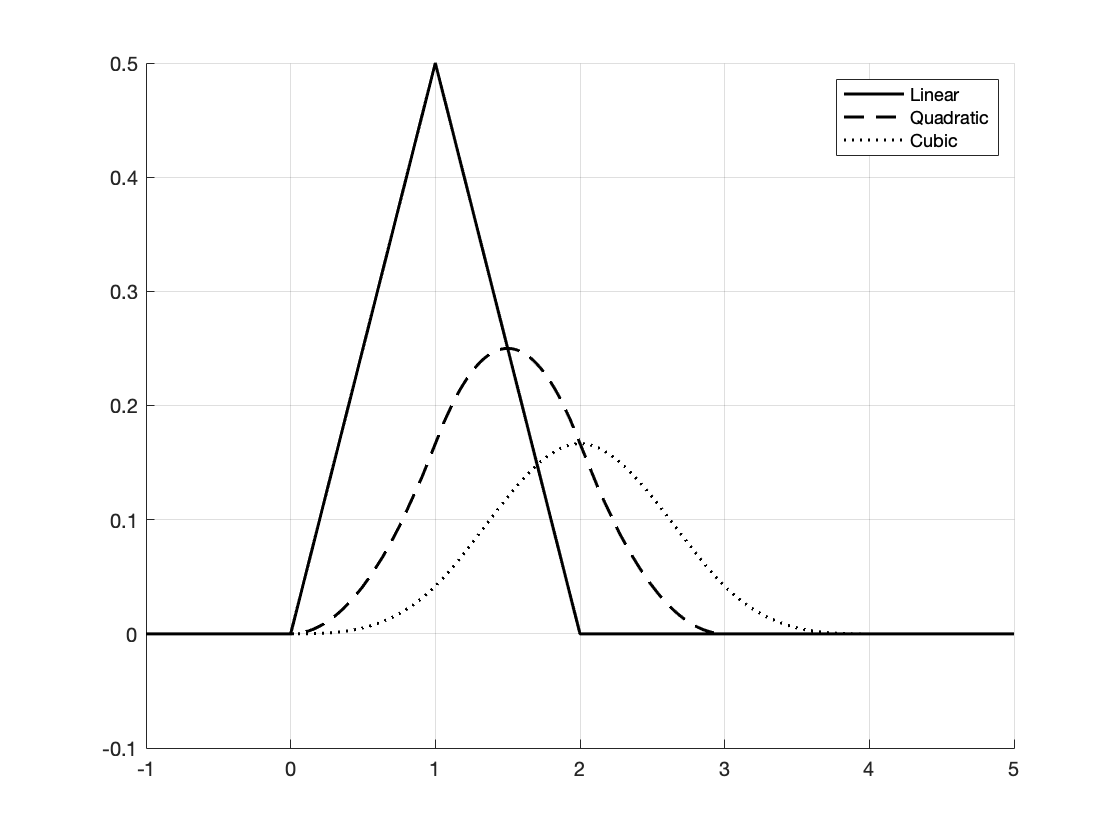
\includegraphics[width=8cm]{/Users/guilhermesalome/Teaching/Duke/Econ890 Matlab - 2019/supporting/matlab_bsplines.png}
\caption{\label{fig:org9c70a67}
Linear, Quadratic and Cubic B-Splines.}
\end{figure}
We constructed splines starting at the knot \(0\).
Observe that the linear spline extends from \(0\) to \(2\), but is zero elsewhere.
The quadratic and cubic splines extend over a slightly longer interval.
We can generate splines starting at other knots, and combine them to create an approximation for some function of interest.
\subsubsection{Example}
\label{sec:orgbcfaa8f}
Let's analyze Runge's example again.
Instead of using Legendre polynomials, we will now use the B-splines to approximate the function in Runge's example.
We begin with a linear B-spline approximation:
\lstset{language=matlab,label= ,caption= ,captionpos=b,firstnumber=1,numbers=left,style=Matlab-editor}
\begin{lstlisting}
% Runge's example: continuous function on interval [-5, 5]
f = @(x) 1./(1+x.^2);
% define B-splines of order 1 (linear)
knots = [-5:5]';
k = 1;
b1 = splineB(knots, 1, k);
b2 = splineB(knots, 2, k);
b3 = splineB(knots, 3, k);
b4 = splineB(knots, 4, k);
b5 = splineB(knots, 5, k);
b6 = splineB(knots, 6, k);
b7 = splineB(knots, 7, k);
b8 = splineB(knots, 8, k);
b9 = splineB(knots, 9, k);
b10 = splineB(knots, 10, k);
B = @(x) [b1(x) b2(x) b3(x) b4(x) b5(x) b6(x) b7(x) b8(x) b9(x) b10(x)];
% Notice that the splines do not work with vector inputs,
% so we will need for-loops to evaluate it.

% Approximate also using the 11 knots
P = zeros(length(knots), 10);
for i = 1:length(knots)
    P(i, :) = B(knots(i));
end
beta = pinv(P'*P)*P'*f(knots);
fhat = @(x) B(x)*beta;
% Visualize
fplot(f, [-5  5]);
hold on;
x = linspace(-5, 5);
fhats = zeros(length(x), 1);
for i = 1:length(fhats)
    fhats(i) = fhat(x(i));
end
plot(x, fhats);
legend(["Original Function", "Approximation"]);
ylim([0 1]);
grid on;
\end{lstlisting}
Observe that the approximation does not suffer from the problems of using a polynomial basis.
The piecewise polynomials are localized, and have little effect on each other.

We can also use a cubic B-spline with the same knots, but we need more observations to approximate the function.
We can also extend the first knots so that the first B-spline does not start at zero.
\lstset{language=matlab,label= ,caption= ,captionpos=b,firstnumber=1,numbers=left,style=Matlab-editor}
\begin{lstlisting}
% Runge's example: continuous function on interval [-5, 5]
f = @(x) 1./(1+x.^2);
% define B-splines of order 1 (linear)
knots = [-7:5]';
k = 3;
b1 = splineB(knots, 1, k);
b2 = splineB(knots, 2, k);
b3 = splineB(knots, 3, k);
b4 = splineB(knots, 4, k);
b5 = splineB(knots, 5, k);
b6 = splineB(knots, 6, k);
b7 = splineB(knots, 7, k);
b8 = splineB(knots, 8, k);
b9 = splineB(knots, 9, k);
b10 = splineB(knots, 10, k);
B = @(x) [b1(x) b2(x) b3(x) b4(x) b5(x) b6(x) b7(x) b8(x) b9(x) b10(x)];
% Notice that the splines do not work with vector inputs,
% so we will need for-loops to evaluate it.

% Approximate also using the 11 knots
obs = linspace(-5, 5)';
P = zeros(length(obs), 10);
for i = 1:length(obs)
    P(i, :) = B(obs(i));
end
beta = pinv(P'*P)*P'*f(obs);
fhat = @(x) B(x)*beta;
% Visualize
fplot(f, [-5  5]);
hold on;
x = linspace(-5, 5);
fhats = zeros(length(x), 1);
for i = 1:length(fhats)
    fhats(i) = fhat(x(i));
end
plot(x, fhats);
legend(["Original Function", "Approximation"]);
ylim([0 1]);
grid on;
\end{lstlisting}
\subsection{Approximating Functions of Many Variables}
\label{sec:org094c394}
We can use the same methodology to approximate a function \(f\) of many variables.
In this case, \(f:\mathbb{R}^n\mapsto\mathbb{R}\), so that \(x\) is now a vector of dimension \(n\).
Let's consider a basis of power functions to approximate \(f\).
Let \(p_k(x)\) denote a power function of degree \(k\) for the vector \(x\).
It consists of all interaction terms between the elements of \(x\), such that the sum of the exponents of each element is equal to \(k\).
For example:
\begin{align*}
p_0(x) &= 1\\
p_1(x) &= \begin{pmatrix}
x_1\\
x_2
\end{pmatrix}\\
p_2(x) &= \begin{pmatrix}
x_1^2\\
x_1x_2\\
x_2^2
\end{pmatrix}\\
p_3(x) &= \begin{pmatrix}
x_1^3\\
x_1^2x_2\\
x_1x_2^2\\
x_2^3
\end{pmatrix}
\end{align*}
Given a choice for the highest order \(k\) of the polynomials, we can define \(p(x)\) as before.
For example, if we choose \(k=2\):
\begin{align*}
  p(x)=\begin{pmatrix}
    1\\
    x_1\\
    x_2\\
    x_1^2\\
    x_1x_2\\
    x_2^2
  \end{pmatrix}
\end{align*}
Then, given a set of observations for \(x\) and \(f(x)\), we can proceed as in Equations \ref{eq:890_matlab_FPbeta}, \ref{eq:890_matlab_sieves_problem}, \ref{eq:890_matlab_ols_solution} and \ref{eq:890_matlab_fhat}.
\subsection{Matlab Functions}
\label{sec:org9e06026}
There are a few functions in Matlab that help with interpolation.
The function \href{https://www.mathworks.com/help/matlab/ref/interp1.html?s\_tid=doc\_ta}{\texttt{interp1}} provides interpolation for 1-dimensional data.
To use it, we must supply observations \(\Set{(x, f(x))}\), a set of points where we want to evaluate the interpolation and the method of interpolation (default is linear).
\lstset{language=matlab,label= ,caption= ,captionpos=b,firstnumber=1,numbers=left,style=Matlab-editor}
\begin{lstlisting}
% Runge's example: continuous function on interval [-5, 5]
f = @(x) 1./(1+x.^2);
x = [-5:5];
eval_at = linspace(-5, 5);
fhat = interp1(x, f(x), eval_at, 'linear');
% Visualize
fplot(f, [-5  5]);
hold on;
plot(eval_at, fhat);
legend(["Original Function", "Approximation"]);
ylim([0 1]);
grid on;
\end{lstlisting}
We can also use piecewise cubic splines with the method \texttt{'pchip'}.
There are also other methods available, see the documentation for a complete list.

The function \href{https://www.mathworks.com/help/matlab/ref/interp2.html}{\texttt{interp2}} allows for interpolation of 2-dimensional data, and works in a similar way to \texttt{interp1}.
The function \href{https://www.mathworks.com/help/matlab/ref/interpn.html}{\texttt{interpn}} extends the interpolation to n-dimensional data.
\section{Integration}
\label{sec:orgcaca6db}
We will discuss three methods for computing integrals numerically: \href{https://en.wikipedia.org/wiki/Newton–Cotes\_formulas}{Newton-Cotes}, \href{https://en.wikipedia.org/wiki/Numerical\_integration\#Quadrature\_rules\_based\_on\_interpolating\_functions}{Quadrature} and \href{https://en.wikipedia.org/wiki/Monte\_Carlo\_integration}{Monte Carlo}.
\subsection{Netwon-Cotes}
\label{sec:org43b98a0}
We want to compute the following integral:
\begin{align*}
\int_a^bf(x)dx
\end{align*}
Assume that we can compute the value of \(f\) at a set of equally spaced points \(x_0=a,x_1,x_2,\dots,x_n=b\).
The idea of Newton-Cotes is to interpolate the function with \href{https://en.wikipedia.org/wiki/Lagrange\_polynomial}{Lagrange polynomials} and the integrate the polynomial.
The approximation yields:
\begin{align*}
f(x)\approx \sum_{i=0}^nf(x_i)l_i(x)
\end{align*}
Where \(l_i\) is a Lagrange polynomial, and the weights multiplying the polynomials only depend on the points \(x0, \dots, x_n\) and on \(f\).
This approximation can now be integrated:
\begin{align*}
\int_a^b f(x)dx&\approx\int_a^b\left(\sum_{i=0}^nf(x_i)l_i(x)\right)\\
&=\sum_{i=0}^n f(x_i)\underbrace{\int_a^bl_i(x)dx}_{w_i}\\
&=\sum_{i=0}^nf(x_i)w_i
\end{align*}
If we use a Lagrange polynomial of order 1 (linear), then we obtain the \href{https://en.wikipedia.org/wiki/Trapezoidal\_rule}{trapezoidal rule}, and the approximation of the integral is simply:
\begin{align*}
\int_a^b f(x)dx\approx\sum_{i=1}^n\frac{f(x_{i-1}) + f(x_i)}{2}(x_i-x_{i-1})
\end{align*}
Since the points are equally spaced, we can simplify the equation above.
Let \(\Delta x\equiv x_i-x_{i-1}\), then:
\begin{align*}
\int_a^b f(x)dx\approx \frac{\Delta x}{2}\left[f(x_0) + 2f(x_1) + 2f(x_2) + \cdots + 2f(x_{n-1}) + f(x_n)\right]
\end{align*}
If we use a higher order Lagrange polynomial to approximate \(f\), then we obtain different weights \(w_i\).

Example:
\lstset{language=matlab,label= ,caption= ,captionpos=b,firstnumber=1,numbers=left,style=Matlab-editor}
\begin{lstlisting}
f = @(x) x.^2;
x = [1:5];
delta_x = x(2) - x(1);
int_f = (2*sum(f(x)) - f(x(1)) - f(x(end)))*(delta_x/2);
\end{lstlisting}
The trapezoidal rule is implemented in Matlab in the function \href{https://www.mathworks.com/help/matlab/ref/trapz.html}{\texttt{trapz}}.
It assumes points are equally spaced with space equal to unit.
\lstset{language=matlab,label= ,caption= ,captionpos=b,firstnumber=1,numbers=left,style=Matlab-editor}
\begin{lstlisting}
x = [1:5];
% equally spaced points, with space = 1
trapz(f(x))
% not equally spaced
x = [1;1.5;2;2.1;3;3.8;5];
trapz(x, f(x))
\end{lstlisting}
\subsection{Quadrature}
\label{sec:org4ff9752}
The Quadrature method extends Newton-Cotes method by choosing the weights \(w_i\) in a special manner.
The idea is to have weights such that the approximation of the integral of \(f\) is actually an equality when \(f\) is a polynomial of some order.
Matlab implements a modified Quadrature method on the function \href{https://www.mathworks.com/help/matlab/ref/integral.html}{\texttt{integral}}.
This modified method also works when the integrand diverges.

To use \texttt{integral}, we need to pass a function handle to the function we want to integrate, and the bounds of integration.
\lstset{language=matlab,label= ,caption= ,captionpos=b,firstnumber=1,numbers=left,style=Matlab-editor}
\begin{lstlisting}
f = @(x) exp(-x);
% integrate over [0 1]
integral(f, 0, 1)
% integrate over [0, infinity)
integral(f, 0, Inf)
% integrate symmetric function over [0 2*pi]
integral(@sin, 0, pi)
integral(@sin, 0, 2*pi)
\end{lstlisting}
\subsection{Monte Carlo}
\label{sec:org228ac69}
The idea of Monte-Carlo integration is to use the law of large numbers to compute the integral of \(f\).
Consider a random variable \(Z\) with a density \(\phi\) defined on the real line.
Then, we can compute the integral of \(f\) in the following way:
\begin{align*}
\int_{-\infty}^{+\infty}f(x)dx &= \int_{-\infty}^{ +\infty}\frac{f(x)}{\phi(x)}\phi(x)dx\\
&= \mathbb{E}_{Z}\left[\frac{f(Z)}{\phi(Z)}\right]
\end{align*}
For example, we could have \(\phi\) be the density of the standard normal distribution.
Now, we can simulate an i.i.d. sample from this density, and approximate the integral via:
\begin{align*}
\int_{-\infty}^{+\infty}f(x)dx\approx\frac{1}{n}\sum_{i=1}^n\frac{f(x_i)}{\phi(z_i)}
\end{align*}
The term on the right-hand side will approximate the true value of the integral with probability one due to the law of large numbers.
Example:
\lstset{language=matlab,label= ,caption= ,captionpos=b,firstnumber=1,numbers=left,style=Matlab-editor}
\begin{lstlisting}
f = @(x) exp(-x.^2);                    % integral = (pi)^0.5
% generate values from the standard normal
x = normrnd(0, 1, 10, 1);
disp(mean(f(x)./normpdf(x)))
% increase number of observations
x = normrnd(0, 1, 1000000, 1);
disp(mean(f(x)./normpdf(x)))
\end{lstlisting}

If the integral is defined over a finite interval, say \([a, b]\), then we can use the uniform distribution over the same interval to generate the i.i.d. sample of \(x_i\)'s.
In this case, let \(\mu(x)=\frac{1}{b-a}\mathds{1}_{[a, b]}(x)\) represent the uniform density over \([a, b]\).
Then:
\begin{align*}
\int_{a}^{b}f(x)dx&=\int_{a}^{b}\frac{f(x)}{\mu(x)}\mu(x)dx\\
&=\mathbb{E}_{U}\left[\frac{f(U)}{\mu(U)}\right]\\
&\approx\frac{1}{n}\sum_{i=1}^n\frac{f(x_i)}{\mu(x_i)}\\
&=\frac{b-a}{n}\sum_{i=1}^nf(x_i)
\end{align*}
Example:
\lstset{language=matlab,label= ,caption= ,captionpos=b,firstnumber=1,numbers=left,style=Matlab-editor}
\begin{lstlisting}
% integrate over [0, 5]
f = @(x) x.^2;
% generate random values over interval [0, 5]
x = unifrnd(0, 5, 10, 1);
int_f = 5*mean(f(x))
% integral approximation converges as we increase number of points
% 100 observations
x = unifrnd(0, 5, 100, 1);
int_f = 5*mean(f(x))
% 1000 observations
x = unifrnd(0, 5, 1000, 1);
int_f = 5*mean(f(x))
% 10000 observations
x = unifrnd(0, 5, 10000, 1);
int_f = 5*mean(f(x))
\end{lstlisting}

This method of integration is very useful for functions of many variables and can be easily made to run in parallel.
\section{Symbolic Math}
\label{sec:org2d1d100}
For this part you will need to install the \href{https://www.mathworks.com/help/symbolic/index.html?s\_tid=CRUX\_lftnav}{Symbolic Math Toolbox}.
We can use the toolbox to do analytical computations, like differentiation, integration, simplification, transformations, and equation solving.
\subsection{Creating Symbolic Variables and Expressions}
\label{sec:orga4b404e}
To create the symbolic variables we use the function \href{https://www.mathworks.com/help/symbolic/sym.html}{\texttt{sym}}.
\lstset{language=matlab,label= ,caption= ,captionpos=b,firstnumber=1,numbers=left,style=Matlab-editor}
\begin{lstlisting}
% clear the workspace
clear all
% create a symbolic number
sym(1/3)
% expressions involving symbols are displayed unindented
sym(pi)
% we can do computations with symbols, and the computations are
% analytical
sin(pi)
sin(sym(pi))
% create a variable
sym('x')                                % unasigned so cannot be reused
sym('x')*sym(pi)
% create a variable and assign it
x = sym('x');
x + 2
% verify the class of x
whos x
\end{lstlisting}
We can create multiple variables at once with the function \href{https://www.mathworks.com/help/symbolic/syms.html}{\texttt{syms}}.
\lstset{language=matlab,label= ,caption= ,captionpos=b,firstnumber=1,numbers=left,style=Matlab-editor}
\begin{lstlisting}
clear all
syms a b c x y
% combine symbolic variables to create expressions
z = (exp(a) + log(b) - c)/(x+y)
\end{lstlisting}
The function \texttt{syms} is a shorthand function for invoking \texttt{sym} multiple times.

We can use \texttt{sym} to create vectors and matrices of symbolic variables.
\lstset{language=matlab,label= ,caption= ,captionpos=b,firstnumber=1,numbers=left,style=Matlab-editor}
\begin{lstlisting}
% pass sym the name and dimension
A = sym('a', [3, 1])
% create a matrix
X = sym('x', [2, 2])

% create symbolic matrix from numeric matrix
Y = [0.25; 1/3; pi; 0.1245];
Y = sym(Y);
\end{lstlisting}

We can use \texttt{syms} with \texttt{sym} to create multiple symbolic variables where the names are numbered:
\lstset{language=matlab,label= ,caption= ,captionpos=b,firstnumber=1,numbers=left,style=Matlab-editor}
\begin{lstlisting}
clear all
% create symbolic variables a
syms(sym('a', [5, 1]))
syms(sym('x', [2, 2]))
\end{lstlisting}

Symbolic expressions can be combined:
\lstset{language=matlab,label= ,caption= ,captionpos=b,firstnumber=1,numbers=left,style=Matlab-editor}
\begin{lstlisting}
clear all
syms x y z
f = x^2 + y^2 + z^2;
g = exp(f^2)/2
% symbolic expressions can be reused by restating them with syms
syms f
f
g
\end{lstlisting}
\subsection{Creating Symbolic Functions}
\label{sec:org0e15d3c}
Symbolic functions are used to perform the analytical computations.
We can create them with \texttt{syms}:
\lstset{language=matlab,label= ,caption= ,captionpos=b,firstnumber=1,numbers=left,style=Matlab-editor}
\begin{lstlisting}
clear all
% create a function f of two variables, x and y
syms f(x, y)
% x and y are symbolic variables
whos x y
% f is a symbolic function
whos f
% assign an expression to f
f(x, y) = x^2 + x*y + y^2;
% we can evaluate the function
f(0, 0)
f(1, 0)
f([1, 2, 3], [-1, -2, -3])
\end{lstlisting}
\subsection{Derivatives}
\label{sec:orgef85bde}
We can use the function \href{https://www.mathworks.com/help/symbolic/diff.html?s\_tid=doc\_ta}{\texttt{diff}} to differentiate a symbolic function.
The function \texttt{diff} returns a symbolic function with the same arguments as the function being differentiated.
\lstset{language=matlab,label= ,caption= ,captionpos=b,firstnumber=1,numbers=left,style=Matlab-editor}
\begin{lstlisting}
syms f(x, y)
f(x, y) = x^3 + 2*x*y + y^2
% differentiate with respect to x
dfdx = diff(f, x)
% evaluate the derivative
dfdx(1, 0)
% differentiate with respect to x again
dfdx2 = diff(dfdx, x)
% equivalent
dfdx2 = diff(f, x, 2)
% differentiate with respect to y and x
dfdyx = diff(f, y, x)
% differentiate with respect to x and y
dfdxy = diff(f, x, y)

% can also differentiate expressions
diff(x^2, x)
diff(x^2, x, 2)
\end{lstlisting}
\subsection{Integral}
\label{sec:org35e8081}
The function \href{https://www.mathworks.com/help/symbolic/performing-symbolic-computations.html}{\texttt{int}} is used to integrate symbolic expressions:
\lstset{language=matlab,label= ,caption= ,captionpos=b,firstnumber=1,numbers=left,style=Matlab-editor}
\begin{lstlisting}
clear all
% specify function
syms f(x)
f(x) = exp(-x^2)
% integrate from -infinity to infinity
int_f = int(f)
% evaluate integral
int_f(1)
% integrate from 0 to 1
int(f, 0, 1)
% specify a multivariate function
syms f(x, y)
f(x, y) = x^3 + x^2*y + x*y^2 + y^3
% integrate with respect to x
int(f, x)
% integrate with respect to y
int(f, y)
% if variable not specified it is implied from first variable
int(f)                                  % same as int(f, x) in this case
% another multivariate function
syms f(x, y) n
f(x, y) = x^n + y^n
int(f, x)
int(f, n)

% if function cannot be integrated, the integral is left unresolved
int(sin(sinh(x)))
\end{lstlisting}
\subsection{Solve Equations}
\label{sec:org34a8df7}
We can use the function \href{https://www.mathworks.com/help/symbolic/solve.html}{\texttt{solve}} to solve symbolic equations:
\lstset{language=matlab,label= ,caption= ,captionpos=b,firstnumber=1,numbers=left,style=Matlab-editor}
\begin{lstlisting}
clear all
% solve equation on one variable
syms x
sol = solve(-x^2 + 2*x + 3 == 0, x)
% sol is still symbolic
whos sol
% if the right-hand side is not specified, then == 0 is implied
sol = solve(-x^2 + 2*x + 3, x)
% solve equations with several variables
syms x y
solve(-3*x^2 + 2*x*y + y^2 == 0, y)
% solve a system of equations
syms x y z
[sol_x, sol_y, sol_z] = solve(z == 4*x, x == y/2, z == x^2 + y^2)
\end{lstlisting}
Matlab implements solvers for more complex equations, as systems of differential equations.
For a complete description, refer to the \href{https://www.mathworks.com/help/symbolic/equation-solving.html}{Equation Solving reference page}.
\subsection{Simplify Expressions}
\label{sec:org53f26ca}
The function \href{https://www.mathworks.com/help/symbolic/simplify.html?s\_tid=doc\_ta}{\texttt{simplify}} can be used to simplify symbolic expressions:
\lstset{language=matlab,label= ,caption= ,captionpos=b,firstnumber=1,numbers=left,style=Matlab-editor}
\begin{lstlisting}
clear all
syms x y
f = sin(x)^2 + cos(x)^2
% simplify expression
simplify(f)
% another example
g = (sym(1) + sqrt(5))/2                % need one symbol at least
simplify(g^2 - g - 1)
\end{lstlisting}
There is no clear way of simplifying a mathematical expression, and the results will vary with the way the symbolic expressions are built.

The function \href{https://www.mathworks.com/help/symbolic/expand.html?s\_tid=doc\_ta}{\texttt{expand}} can be used to expand symbolic expressions:
\lstset{language=matlab,label= ,caption= ,captionpos=b,firstnumber=1,numbers=left,style=Matlab-editor}
\begin{lstlisting}
% expand polynomial
f = (x-2)*(x-3)*(y-2)
f_expanded = expand(f)
% simplify expanded expression
simplify(f_expanded)
% expand expression
expand((x-1)*(x+1))
\end{lstlisting}

The function \href{https://www.mathworks.com/help/symbolic/factor.html?s\_tid=doc\_ta}{\texttt{factor}} can be used to factor expressions:
\lstset{language=matlab,label= ,caption= ,captionpos=b,firstnumber=1,numbers=left,style=Matlab-editor}
\begin{lstlisting}
f = (x-2)*(x-3)*(y-2)
f_expanded = expand(f)
factor(f_expanded)
\end{lstlisting}
The function \href{https://www.mathworks.com/help/symbolic/horner.html?s\_tid=doc\_ta}{\texttt{horner}} factors polynomials to a form that is efficient for computation.
\lstset{language=matlab,label= ,caption= ,captionpos=b,firstnumber=1,numbers=left,style=Matlab-editor}
\begin{lstlisting}
horner(f)
\end{lstlisting}
\subsection{Substitutions}
\label{sec:org7cd7a50}
While symbolic functions can be evaluated as a regular function, symbolic expressions are not functions, and to be evaluated we need to use the function \href{https://www.mathworks.com/help/symbolic/subs.html?s\_tid=doc\_ta}{\texttt{subs}}.
\lstset{language=matlab,label= ,caption= ,captionpos=b,firstnumber=1,numbers=left,style=Matlab-editor}
\begin{lstlisting}
syms x y
f = (x-2)*(x-3)*(y-2)
f_expanded = expand(f)
% substitute x for 3
subs(f_expanded, x, 3)
% substitute y for 0
subs(f_expanded, y, 0)
% substitute a variable for another
subs(f_expanded, y, x)

% also applies to matrices
% create matrix with notation xij
X = sym('x%d%d', [3, 3])
subs(X, 'x11', 5)
\end{lstlisting}
\subsection{Plotting}
\label{sec:orgcbfa39b}
To plot symbolic expressions and functions we can use the functions:
\begin{itemize}
\item \href{https://www.mathworks.com/help/symbolic/fplot.html}{\texttt{fplot}} for 2-D plots
\item \href{https://www.mathworks.com/help/symbolic/fplot3.html}{\texttt{fplot3}} for 3-D curves
\item \href{https://www.mathworks.com/help/symbolic/fsurf.html}{\texttt{fsurf}} for surfaces
\item \href{https://www.mathworks.com/help/symbolic/fcontour.html}{\texttt{fcontour}} for countor plots
\end{itemize}
There is also a function for plots on polar coordinates (\href{https://www.mathworks.com/help/symbolic/ezpolar.html}{\texttt{ezpolar}}) and one for mesh plots (\href{https://www.mathworks.com/help/symbolic/fmesh.html}{\texttt{fmesh}}).
\subsection{Assumptions}
\label{sec:orgf2939f4}
The symbolic variables are by default assumed to be complex variables.
We can use the function \href{https://www.mathworks.com/help/symbolic/assumptions.html}{\texttt{assumptions}} to verify it.
\lstset{language=matlab,label= ,caption= ,captionpos=b,firstnumber=1,numbers=left,style=Matlab-editor}
\begin{lstlisting}
% create variable
syms z
% verify it is complex
% should return empty symbolic object
assumptions(z)
\end{lstlisting}
We can add assumptions to a symbolic variable with the function \href{https://www.mathworks.com/help/symbolic/assume.html}{\texttt{assume}}.
\lstset{language=matlab,label= ,caption= ,captionpos=b,firstnumber=1,numbers=left,style=Matlab-editor}
\begin{lstlisting}
syms x
assume(x >= 0)
% assumptions impact the behavior of other functions
syms f(x)
f(x) = x^2
fplot(f)
% solve for roots
solve(-2*x^2 + 3*x + 3 == 0, x)
\end{lstlisting}
Additional assumptions can be added to the same symbolic variable with the function \href{https://www.mathworks.com/help/symbolic/assumealso.html?s\_tid=doc\_ta}{\texttt{assumeAlso}}.

To clear assumptions restate the symbolic variable or use \texttt{assume} with the \texttt{'clear'} option:
\lstset{language=matlab,label= ,caption= ,captionpos=b,firstnumber=1,numbers=left,style=Matlab-editor}
\begin{lstlisting}
% clear assumptions
assumptions(x)
syms x
assumptions(x)                          % now empty

assume(x, 'integer')
assumptions(x)
assume(x, 'clear')
assumptions(X=x)
\end{lstlisting}
\section{Assignment}
\label{sec:org6aa77ab}
\begin{problem}
Consider a deterministic growth model, where an agent decides between consumption (\(c_t\)) and investment in capital (\(k_t\)), while maximizing his utility.
We can write this problem as:
\begin{align*}
  \max&\sum_{t=0}^{\infty}\beta^tU(c_t)\\
  \text{subject to }&
                      \begin{cases}
                        k_{t+1} = k_t^{\alpha} - c_t + (1-\delta)k_t, \forall t >= 0\\
                        k_0 > 0
                      \end{cases}
\end{align*}
Write the problem as a \href{https://en.wikipedia.org/wiki/Bellman\_equation}{Bellman equation}.
You should obtain an equation similar to:
\begin{align*}
V(k) = \max_{k'}{f(k, k') + \beta V(k')}
\end{align*}
\end{problem}

\begin{problem}
(continuation of previous problem)
Consider \(U(c; \sigma)=\frac{c^{1-\sigma}-1}{1-\sigma}\).
Obtain the Euler equation for this problem in terms of the consumption \(c\).
\end{problem}

\begin{problem}
(continuation of previous problem) (Optional)
Use the Symbolic toolbox to obtain the Euler equation for this problem in terms of the consumption \(c\).
\end{problem}

\begin{problem}
(continuation of previous problem)
Assume we are in a steady state (\(c=c'=c^*\) and \(k=k'=k^*\)), then use the Euler equation to compute the steady state value of \(k\).
\end{problem}

\begin{problem}
(continuation of previous problem)
Solve the problem by Value Function Iteration.
Consider \(\sigma=2\), \(\beta=0.95\), \(\delta=0.1\) and \(\alpha=0.33\).
Use the steady state value of \(k\) to create a grid for the possible values of \(k\), say \(100\) points between \(0.25 k^*\) and \(1.75 k^*\).
Start with a guess for \(V\) over the grid, for example \(V(k)=0\) for all \(k\) in the grid.
Use the Matlab minimization function to solve for \(k\).
You may want to add the constraint that \(c\) should always be positive.
\end{problem}

\begin{problem}
(continuation of previous problem)
Plot the value for different capital levels. Interpret.
\end{problem}

\begin{problem}
(continuation of previous problem)
Plot the optimal policy function (choice of \(k'\) given \(k\)).
Plot a 45 degree line with the policy function.
Interpret in terms of a steady state.
\end{problem}
\newpage
\printbibliography
\newpage
\end{document}